\documentclass[tikz,border=0pt]{standalone}

\definecolor{skytop}{RGB}{5,8,32}
\definecolor{skymid}{RGB}{14,26,74}
\definecolor{skylow}{RGB}{40,52,106}
\definecolor{starcol}{RGB}{255,255,238}
\definecolor{hanabigold}{RGB}{255,208,96}
\definecolor{hanabipink}{RGB}{255,112,168}
\definecolor{hanabicyan}{RGB}{124,232,255}
\definecolor{hanabigreen}{RGB}{158,255,168}
\definecolor{lanternred}{RGB}{226,76,54}
\definecolor{lanterncream}{RGB}{255,226,168}
\definecolor{lanternglow}{RGB}{255,192,104}
\definecolor{stallwood}{RGB}{26,22,44}
\definecolor{stallroof}{RGB}{34,28,52}
\definecolor{treecol}{RGB}{16,20,46}
\definecolor{groundcol}{RGB}{20,18,38}
\definecolor{silhouette}{RGB}{8,7,20}
\definecolor{watertop}{RGB}{28,40,86}
\definecolor{waterbot}{RGB}{10,14,40}

% firework : #1 x  #2 y  #3 scale  #4 color   (unit radius = 1)
\newcommand{\hanabi}[4]{%
  \begin{scope}[shift={(#1,#2)},scale=#3]
    \foreach \g in {1.25,1.05,0.85,0.65,0.45,0.25}{%
      \fill[#4,opacity=0.04] (0,0) circle (\g);
    }
    \foreach \a in {0,30,60,90,120,150,180,210,240,270,300,330}{%
      \draw[#4!85!white,line width=0.8pt,line cap=round] (\a:0.12) -- (\a:0.62);
      \draw[#4,opacity=0.55,line width=0.6pt,line cap=round] (\a:0.62) -- (\a:0.97);
      \fill[#4!45!white,opacity=0.9] (\a:1.0) circle (0.04);
      \fill[white,opacity=0.4] (\a:1.0) circle (0.017);
    }
    \foreach \a in {15,45,75,105,135,165,195,225,255,285,315,345}{%
      \draw[#4!80!white,opacity=0.8,line width=0.7pt,line cap=round] (\a:0.10) -- (\a:0.52);
      \draw[#4,opacity=0.45,line width=0.5pt,line cap=round] (\a:0.52) -- (\a:0.80);
      \fill[#4!45!white,opacity=0.85] (\a:0.83) circle (0.033);
    }
    \foreach \a in {0,60,120,180,240,300}{%
      \draw[#4!55!white,opacity=0.6,line width=0.5pt,line cap=round] (\a:0.06) -- (\a:0.34);
      \fill[white,opacity=0.45] (\a:0.36) circle (0.022);
    }
    \fill[white,opacity=0.6] (0,0) circle (0.08);
  \end{scope}
}

% small distant burst : #1 x  #2 y  #3 scale  #4 color
\newcommand{\kohanabi}[4]{%
  \begin{scope}[shift={(#1,#2)},scale=#3]
    \foreach \g in {1.2,0.9,0.6,0.3}{\fill[#4,opacity=0.04] (0,0) circle (\g);}
    \foreach \a in {0,45,90,135,180,225,270,315}{%
      \draw[#4,opacity=0.7,line width=0.5pt,line cap=round] (\a:0.08) -- (\a:0.9);
      \fill[#4!50!white,opacity=0.8] (\a:0.95) circle (0.035);
    }
    \foreach \a in {22,67,112,157,202,247,292,337}{%
      \draw[#4,opacity=0.5,line width=0.4pt,line cap=round] (\a:0.08) -- (\a:0.65);
      \fill[#4!50!white,opacity=0.7] (\a:0.70) circle (0.026);
    }
    \fill[white,opacity=0.45] (0,0) circle (0.07);
  \end{scope}
}

% paper lantern : #1 x  #2 y  #3 scale  #4 body color
\newcommand{\chochin}[4]{%
  \begin{scope}[shift={(#1,#2)},scale=#3]
    \foreach \g in {1.6,1.3,1.0,0.7}{\fill[lanternglow,opacity=0.06] (0,0) circle (\g);}
    \fill[stallwood] (-0.16,0.50) rectangle (0.16,0.60);
    \fill[#4] (0,0) ellipse (0.34 and 0.52);
    \fill[#4!65!lanterncream,opacity=0.6] (0,0.02) ellipse (0.22 and 0.38);
    \fill[lanterncream,opacity=0.8] (0,0.03) ellipse (0.11 and 0.24);
    \draw[stallwood,opacity=0.3,line width=0.4pt] (-0.257,-0.34) -- (0.257,-0.34);
    \draw[stallwood,opacity=0.3,line width=0.4pt] (-0.321,-0.17) -- (0.321,-0.17);
    \draw[stallwood,opacity=0.3,line width=0.4pt] (-0.34,0) -- (0.34,0);
    \draw[stallwood,opacity=0.3,line width=0.4pt] (-0.321,0.17) -- (0.321,0.17);
    \draw[stallwood,opacity=0.3,line width=0.4pt] (-0.257,0.34) -- (0.257,0.34);
    \fill[stallwood] (-0.16,-0.60) rectangle (0.16,-0.50);
    \fill[lanternglow,opacity=0.3] (0,-0.68) ellipse (0.2 and 0.09);
  \end{scope}
}

% festival stall : #1 x center  #2 base y  #3 scale
\newcommand{\yatai}[3]{%
  \begin{scope}[shift={(#1,#2)},scale=#3]
    \foreach \g in {1.5,1.2,0.9,0.6,0.3}{%
      \fill[lanternglow,opacity=0.04] (0,0.7) ellipse ({\g} and {\g});
    }
    \fill[stallwood] (-1.1,0) rectangle (1.1,0.62);
    \fill[lanternglow,opacity=0.18] (-1.02,0.62) rectangle (1.02,0.70);
    \fill[stallwood] (-1.1,0) rectangle (-1.0,1.3);
    \fill[stallwood] (1.0,0) rectangle (1.1,1.3);
    \fill[stallroof] (-1.38,1.3) -- (1.38,1.3) -- (1.16,1.72) -- (-1.16,1.72) -- cycle;
    \foreach \t in {-1.38,-1.08,-0.78,-0.48,-0.18,0.12,0.42,0.72,1.02}{%
      \fill[lanternred,opacity=0.85] (\t,1.08) rectangle ({\t+0.15},1.3);
      \fill[lanterncream,opacity=0.8] ({\t+0.15},1.08) rectangle ({\t+0.3},1.3);
    }
    \fill[stallwood] (-1.38,1.04) rectangle (1.38,1.08);
    \fill[lanternglow,opacity=0.10] (-1.0,0.70) rectangle (1.0,1.04);
  \end{scope}
}

% standing person : #1 x  #2 base y  #3 scale
\newcommand{\personA}[3]{%
  \begin{scope}[shift={(#1,#2)},scale=#3]
    \fill[silhouette] (-0.17,0) -- (0.17,0) -- (0.13,0.52) -- (-0.13,0.52) -- cycle;
    \fill[silhouette] (-0.15,0.48) -- (0.15,0.48) -- (0.11,0.80) -- (-0.11,0.80) -- cycle;
    \fill[silhouette] (-0.22,0.44) rectangle (-0.13,0.76);
    \fill[silhouette] (0.13,0.44) rectangle (0.22,0.76);
    \fill[silhouette] (0,0.92) circle (0.105);
    \draw[hanabigold,opacity=0.2,line width=0.5pt] (0,0.92) circle (0.112);
    \draw[lanternglow,opacity=0.16,line width=0.5pt] (-0.15,0.49) -- (0.15,0.49);
  \end{scope}
}

% yukata figure with hair bun and round fan : #1 x  #2 base y  #3 scale
\newcommand{\personY}[3]{%
  \begin{scope}[shift={(#1,#2)},scale=#3]
    \fill[silhouette] (-0.22,0) -- (0.22,0) -- (0.13,0.56) -- (-0.13,0.56) -- cycle;
    \fill[silhouette] (-0.14,0.52) -- (0.14,0.52) -- (0.10,0.80) -- (-0.10,0.80) -- cycle;
    \fill[silhouette] (0.10,0.50) -- (0.24,0.64) -- (0.20,0.71) -- (0.07,0.60) -- cycle;
    \fill[silhouette] (0,0.92) circle (0.10);
    \fill[silhouette] (0.08,1.01) circle (0.055);
    \draw[hanabipink,opacity=0.22,line width=0.5pt] (0,0.92) circle (0.107);
    \draw[silhouette,line width=1.2pt] (0.24,0.64) -- (0.32,0.76);
    \fill[silhouette] (0.36,0.84) circle (0.10);
    \draw[lanternglow,opacity=0.22,line width=0.5pt] (0.36,0.84) circle (0.105);
  \end{scope}
}

% child holding a lit lantern : #1 x  #2 base y  #3 scale
\newcommand{\personK}[3]{%
  \begin{scope}[shift={(#1,#2)},scale=#3]
    \fill[silhouette] (-0.15,0) -- (0.15,0) -- (0.11,0.42) -- (-0.11,0.42) -- cycle;
    \fill[silhouette] (-0.12,0.38) -- (0.12,0.38) -- (0.09,0.62) -- (-0.09,0.62) -- cycle;
    \fill[silhouette] (0,0.74) circle (0.095);
    \draw[silhouette,line width=1.1pt] (-0.10,0.56) -- (-0.26,0.44);
    \draw[silhouette,line width=0.6pt] (-0.26,0.44) -- (-0.26,0.32);
    \foreach \g in {0.28,0.21,0.14,0.07}{%
      \fill[lanternglow,opacity=0.10] (-0.26,0.20) circle (\g);
    }
    \fill[lanternred] (-0.26,0.20) ellipse (0.09 and 0.13);
    \fill[lanterncream,opacity=0.85] (-0.26,0.20) ellipse (0.045 and 0.075);
    \draw[lanternglow,opacity=0.3,line width=0.5pt] (0,0.74) circle (0.102);
  \end{scope}
}

\begin{document}
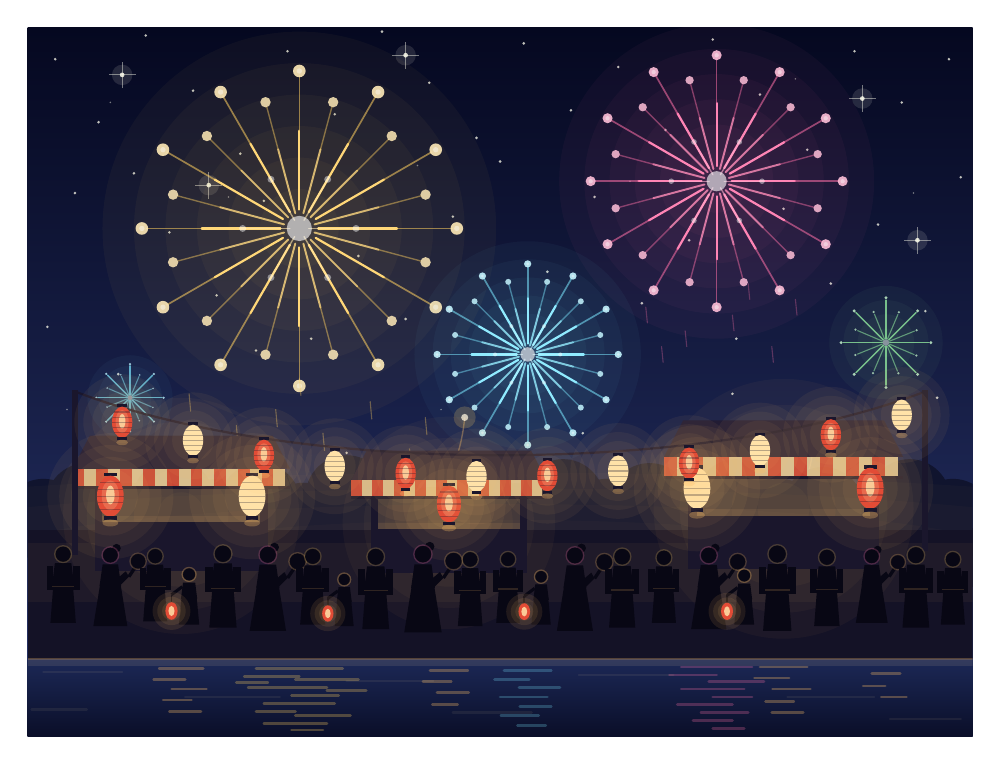
\begin{tikzpicture}
\clip (0,0) rectangle (12,9);

% ---------------- night sky ----------------
\shade[top color=skytop,middle color=skymid,bottom color=skylow]
  (0,0) rectangle (12,9);

% ---------------- stars ----------------
\foreach \px/\py in {0.35/8.6,0.9/7.8,1.5/8.9,2.1/8.2,2.7/7.4,3.3/8.7,
  3.9/7.9,4.5/8.95,5.1/8.3,5.7/7.6,6.3/8.8,6.9/7.95,7.5/8.5,
  8.1/7.7,8.7/8.85,9.3/8.15,9.9/7.45,10.5/8.7,11.1/8.05,11.7/8.6,
  0.6/6.9,1.8/6.4,2.4/5.6,3.0/6.8,4.2/6.1,4.8/5.3,5.4/6.6,
  6.6/5.9,7.2/6.85,7.8/5.5,8.4/6.3,9.0/5.05,9.6/6.7,10.2/5.75,
  10.8/6.5,11.4/5.4,0.25/5.2,1.15/4.6,2.05/3.9,2.9/4.9,4.05/3.6,
  7.05/3.85,11.55/4.3,0.75/3.5,11.85/7.1,3.6/5.05,6.0/7.3,
  8.95/4.35,10.45/3.75,1.35/7.15}{%
  \fill[starcol,opacity=0.75] (\px,\py) circle (0.018);
}
\foreach \px/\py in {1.05/8.05,2.55/6.85,4.95/7.25,7.65/7.05,9.75/8.35,
  11.25/6.9,0.5/4.15,5.25/4.15,8.25/3.4,3.15/3.35}{%
  \fill[starcol,opacity=0.45] (\px,\py) circle (0.011);
}
\foreach \px/\py in {1.2/8.4,4.8/8.65,10.6/8.1,2.3/7.0,11.3/6.3}{%
  \begin{scope}[shift={(\px,\py)}]
    \fill[starcol,opacity=0.85] (0,0) circle (0.03);
    \draw[starcol,opacity=0.45,line width=0.4pt] (-0.17,0) -- (0.17,0);
    \draw[starcol,opacity=0.45,line width=0.4pt] (0,-0.17) -- (0,0.17);
    \fill[starcol,opacity=0.12] (0,0) circle (0.13);
  \end{scope}
}

% ---------------- fireworks ----------------
\hanabi{3.45}{6.45}{2.0}{hanabigold}
\hanabi{8.75}{7.05}{1.6}{hanabipink}
\hanabi{6.35}{4.85}{1.15}{hanabicyan}
\kohanabi{10.9}{5.0}{0.6}{hanabigreen}
\kohanabi{1.3}{4.3}{0.45}{hanabicyan}

% falling embers
\foreach \p in {(2.05,4.35),(2.65,3.95),(3.15,4.15),(3.75,3.85),(4.35,4.25),
  (4.85,3.65),(2.35,3.55),(4.15,3.35),(3.45,4.55),(5.05,4.05)}{%
  \draw[hanabigold,opacity=0.35,line width=0.4pt,line cap=round]
    \p -- ++(0.02,-0.22);
}
\foreach \p in {(7.85,5.45),(8.35,5.15),(8.95,5.35),(9.45,4.95),(9.15,5.75),
  (8.05,4.95),(9.75,5.55)}{%
  \draw[hanabipink,opacity=0.3,line width=0.4pt,line cap=round]
    \p -- ++(0.02,-0.2);
}

% rising shells
\draw[lanternglow,opacity=0.35,line width=0.5pt]
  (5.05,2.6) .. controls (5.3,3.2) and (5.5,3.5) .. (5.55,4.05);
\fill[white,opacity=0.75] (5.55,4.05) circle (0.045);
\fill[hanabigold,opacity=0.2] (5.55,4.05) circle (0.14);
\draw[lanternglow,opacity=0.3,line width=0.5pt]
  (9.6,2.62) .. controls (9.8,3.05) and (9.95,3.3) .. (9.98,3.72);
\fill[white,opacity=0.7] (9.98,3.72) circle (0.038);
\fill[hanabigold,opacity=0.18] (9.98,3.72) circle (0.12);

% ---------------- distant treeline ----------------
\foreach \p in {(0.2,2.75),(0.75,2.95),(1.3,2.7),(1.85,3.0),(2.4,2.75),
  (2.95,2.95),(3.5,2.7),(4.05,3.05),(4.6,2.8),(5.15,2.65),(5.7,2.95),
  (6.25,2.7),(6.8,3.0),(7.35,2.75),(7.9,2.95),(8.45,2.65),(9.0,3.0),
  (9.55,2.75),(10.1,2.9),(10.65,2.7),(11.2,3.0),(11.75,2.75)}{%
  \fill[treecol] \p circle (0.52);
}
\foreach \p in {(0.5,2.6),(1.6,2.55),(2.7,2.6),(3.8,2.55),(4.9,2.6),(6.0,2.55),
  (7.1,2.6),(8.2,2.55),(9.3,2.6),(10.4,2.55),(11.5,2.6)}{%
  \fill[treecol] \p circle (0.36);
}
\fill[treecol] (0,1.9) rectangle (12,2.65);

% warm haze along the horizon
\foreach \g in {1,2,3,4,5}{%
  \fill[lanternglow,opacity=0.022] (6,2.35) ellipse ({2.1*\g} and {0.2*\g});
}

% ---------------- ground ----------------
\fill[groundcol] (0,0.98) rectangle (12,2.62);
\fill[lanternglow,opacity=0.05] (0,1.7) rectangle (12,2.45);

% ---------------- stalls and their lanterns ----------------
\yatai{1.95}{2.1}{1.0}
\yatai{5.35}{2.08}{0.9}
\yatai{9.6}{2.12}{1.1}
\chochin{1.05}{3.05}{0.5}{lanternred}
\chochin{2.85}{3.05}{0.5}{lanterncream}
\chochin{5.35}{2.95}{0.45}{lanternred}
\chochin{8.5}{3.15}{0.5}{lanterncream}
\chochin{10.7}{3.15}{0.5}{lanternred}

% ---------------- lantern garland ----------------
\draw[stallwood,line width=2.2pt] (0.6,2.3) -- (0.6,4.4);
\draw[stallwood,line width=2.2pt] (11.4,2.35) -- (11.4,4.4);
\draw[stallwood,opacity=0.9,line width=0.8pt]
  (0.6,4.38) .. controls (3.4,3.3) and (8.6,3.3) .. (11.4,4.38);
\foreach \x/\y in {1.2/4.19,2.1/3.96,3.0/3.77,3.9/3.63,4.8/3.54,5.7/3.5,
  6.6/3.51,7.5/3.57,8.4/3.67,9.3/3.83,10.2/4.03,11.1/4.28}{%
  \draw[stallwood,line width=0.6pt] (\x,\y) -- (\x,{\y-0.2});
  \fill[stallwood] ({\x-0.03},{\y-0.22}) rectangle ({\x+0.03},{\y-0.18});
}
\foreach \x/\y in {1.2/3.99,3.0/3.57,4.8/3.34,6.6/3.31,8.4/3.47,10.2/3.83}{%
  \chochin{\x}{\y}{0.38}{lanternred}
}
\foreach \x/\y in {2.1/3.76,3.9/3.43,5.7/3.3,7.5/3.37,9.3/3.63,11.1/4.08}{%
  \chochin{\x}{\y}{0.38}{lanterncream}
}

% ---------------- crowd silhouettes ----------------
\personA{0.45}{1.44}{0.95}
\personY{1.05}{1.4}{0.98}
\personA{1.62}{1.46}{0.9}
\personK{2.05}{1.42}{0.86}
\personA{2.48}{1.38}{1.02}
\personY{3.05}{1.34}{1.05}
\personA{3.62}{1.42}{0.94}
\personK{4.02}{1.4}{0.8}
\personA{4.42}{1.36}{1.0}
\personY{5.02}{1.32}{1.08}
\personA{5.62}{1.4}{0.92}
\personA{6.1}{1.44}{0.88}
\personK{6.52}{1.42}{0.82}
\personY{6.95}{1.34}{1.04}
\personA{7.55}{1.38}{0.98}
\personA{8.08}{1.44}{0.9}
\personY{8.65}{1.36}{1.02}
\personK{9.1}{1.42}{0.84}
\personA{9.52}{1.34}{1.06}
\personA{10.15}{1.4}{0.95}
\personY{10.72}{1.44}{0.92}
\personA{11.28}{1.38}{1.0}
\personA{11.75}{1.42}{0.9}

% ---------------- river with reflections ----------------
\shade[top color=watertop,bottom color=waterbot] (0,0) rectangle (12,0.98);
\draw[lanternglow,opacity=0.28,line width=0.9pt] (0,0.98) -- (12,0.98);
\draw[lanterncream,opacity=0.1,line width=2.4pt] (0,0.93) -- (12,0.93);

\foreach \x/\y/\w in {3.45/0.86/0.55,3.1/0.76/0.35,3.8/0.72/0.4,3.3/0.62/0.5,
  3.65/0.52/0.3,3.45/0.42/0.45,3.15/0.32/0.25,3.75/0.26/0.35,3.4/0.16/0.4,
  3.55/0.08/0.2,2.85/0.68/0.2,4.05/0.58/0.25}{%
  \draw[hanabigold,opacity=0.28,line width=1.0pt,line cap=round]
    ({\x-\w},\y) -- ({\x+\w},\y);
}
\foreach \x/\y/\w in {8.75/0.88/0.45,8.45/0.78/0.3,9.0/0.7/0.35,8.7/0.6/0.4,
  8.95/0.5/0.25,8.6/0.4/0.35,8.85/0.3/0.3,8.7/0.2/0.25,8.9/0.1/0.2}{%
  \draw[hanabipink,opacity=0.26,line width=1.0pt,line cap=round]
    ({\x-\w},\y) -- ({\x+\w},\y);
}
\foreach \x/\y/\w in {6.35/0.84/0.3,6.15/0.72/0.22,6.5/0.62/0.26,6.3/0.5/0.3,
  6.45/0.38/0.2,6.25/0.26/0.24,6.4/0.14/0.18}{%
  \draw[hanabicyan,opacity=0.24,line width=1.0pt,line cap=round]
    ({\x-\w},\y) -- ({\x+\w},\y);
}
\foreach \x/\y/\w in {1.95/0.86/0.28,1.8/0.72/0.2,2.05/0.6/0.22,1.9/0.46/0.18,
  2.0/0.32/0.2,5.35/0.84/0.24,5.2/0.7/0.18,5.4/0.56/0.2,5.3/0.4/0.16,
  9.6/0.88/0.3,9.45/0.74/0.22,9.7/0.6/0.24,9.55/0.44/0.18,9.65/0.3/0.2,
  10.9/0.8/0.18,10.75/0.64/0.14,11.0/0.5/0.16}{%
  \draw[lanternglow,opacity=0.3,line width=1.0pt,line cap=round]
    ({\x-\w},\y) -- ({\x+\w},\y);
}
\foreach \x/\y/\w in {0.7/0.82/0.5,2.6/0.5/0.6,4.6/0.7/0.55,5.9/0.3/0.5,
  7.6/0.78/0.6,10.2/0.5/0.55,11.4/0.22/0.45,0.4/0.34/0.35}{%
  \draw[lanterncream,opacity=0.07,line width=0.9pt,line cap=round]
    ({\x-\w},\y) -- ({\x+\w},\y);
}

\end{tikzpicture}
\end{document}
